
% !TeX spellcheck = en_GB
\documentclass{beamer}
\usepackage[utf8]{inputenc}
 \usetheme{antibes}
 \usepackage{movie15}
 \usepackage{graphicx}
 \usepackage{hyperref}
 \hypersetup{
 	colorlinks=true,
 	linkcolor=blue,
 	filecolor=magenta,      
 	urlcolor=cyan,
 }
 
 \urlstyle{same}
 \title[Karsten Moholt Digital] %optional
 {Data science in predictive maintenance }
 
 \subtitle{A short story}
 
 \author[] % (optional, for multiple authors)
 {Yapi Donatien Achou}
 
% \institute[VFU] % (optional)
% {
% 	\inst{1}%
% 	Faculty of Physics\\
% 	Very Famous University
% 	\and
% 	\inst{2}%
% 	Faculty of Chemistry\\
% 	Very Famous University
% }
 
 %\date[VLC 2013] % (optional)
 %{Very Large Conference, April 2013}
 
 \logo{
\includegraphics[height=1.5cm]{km-logo.png}}
 
 
\begin{document}
 
\frame{\titlepage}
 
\begin{frame}
\frametitle{What is data science}
\begin{figure}[H]
	\centering
	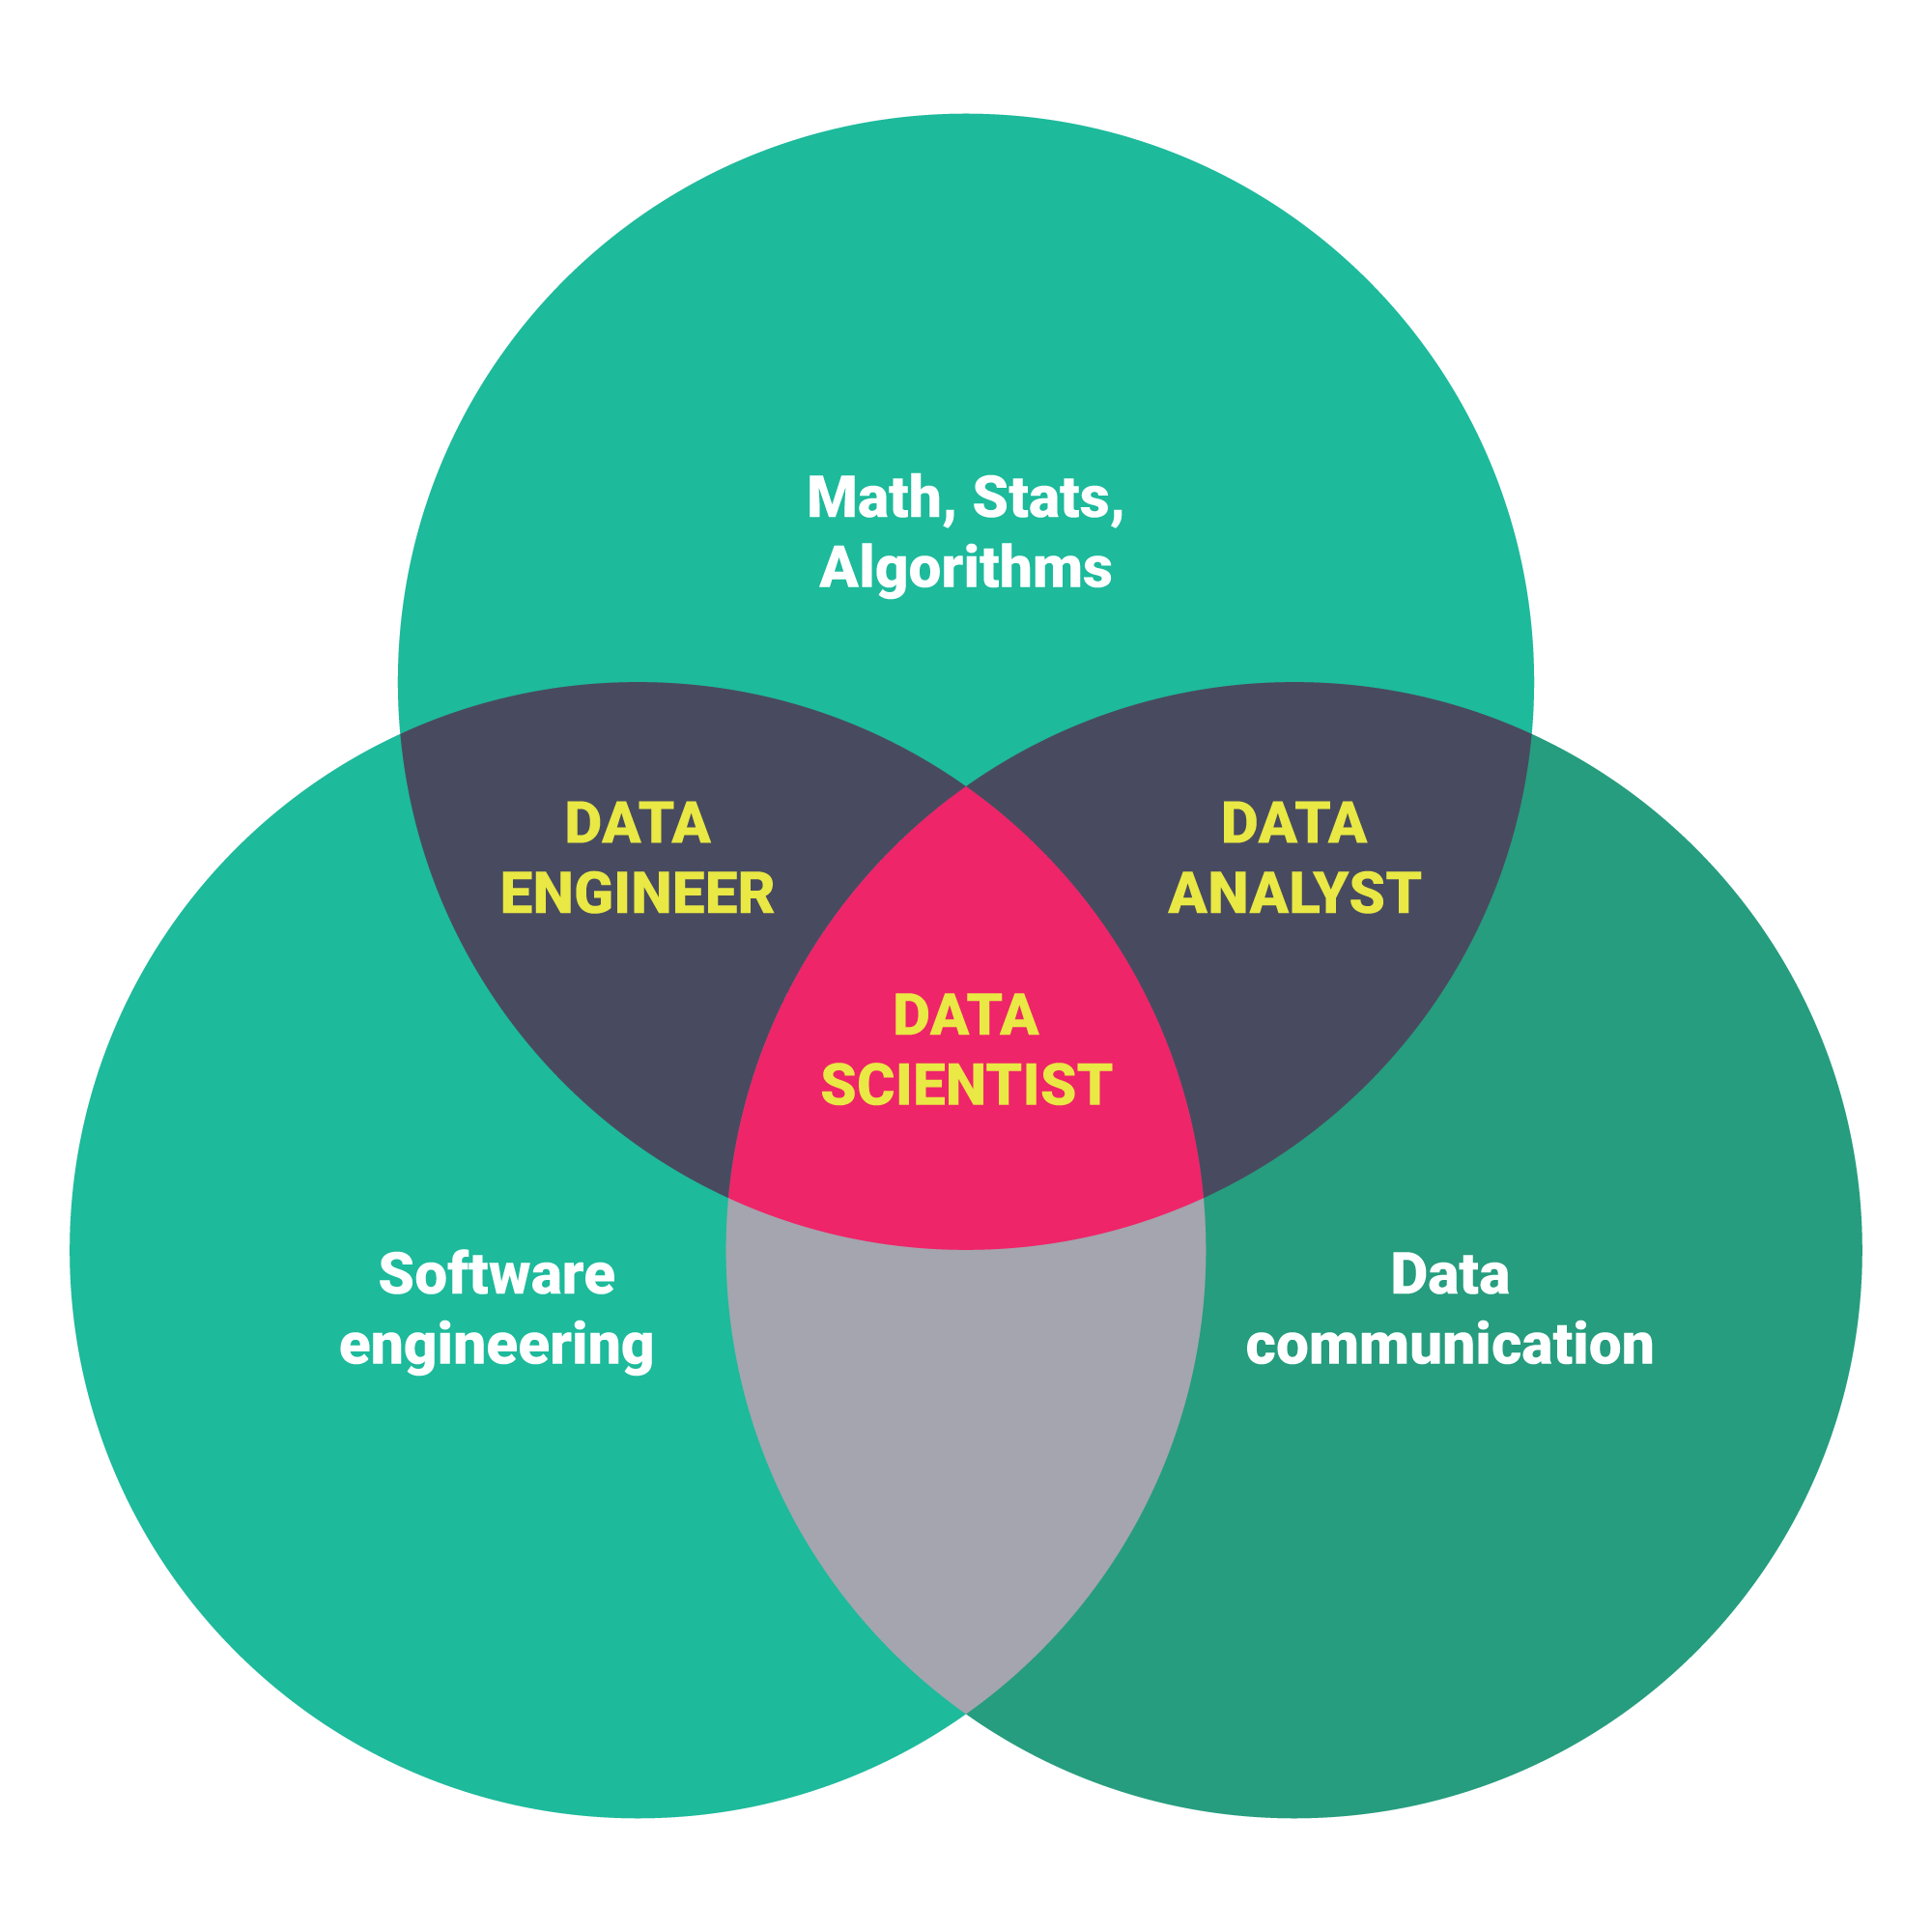
\includegraphics[width=0.5\linewidth]{datascience2}
	%\caption{}
	%\label{fig:datascience}
\end{figure}
\end{frame}
%%%%%%%%%%%%%%%%%%%%%%%%%%%%%%%%%%%%%%%%%%%%%%%%%%%%%%%%%
\begin{frame}
	\frametitle{Data science pipeline}
	\begin{figure}[H]
		\centering
		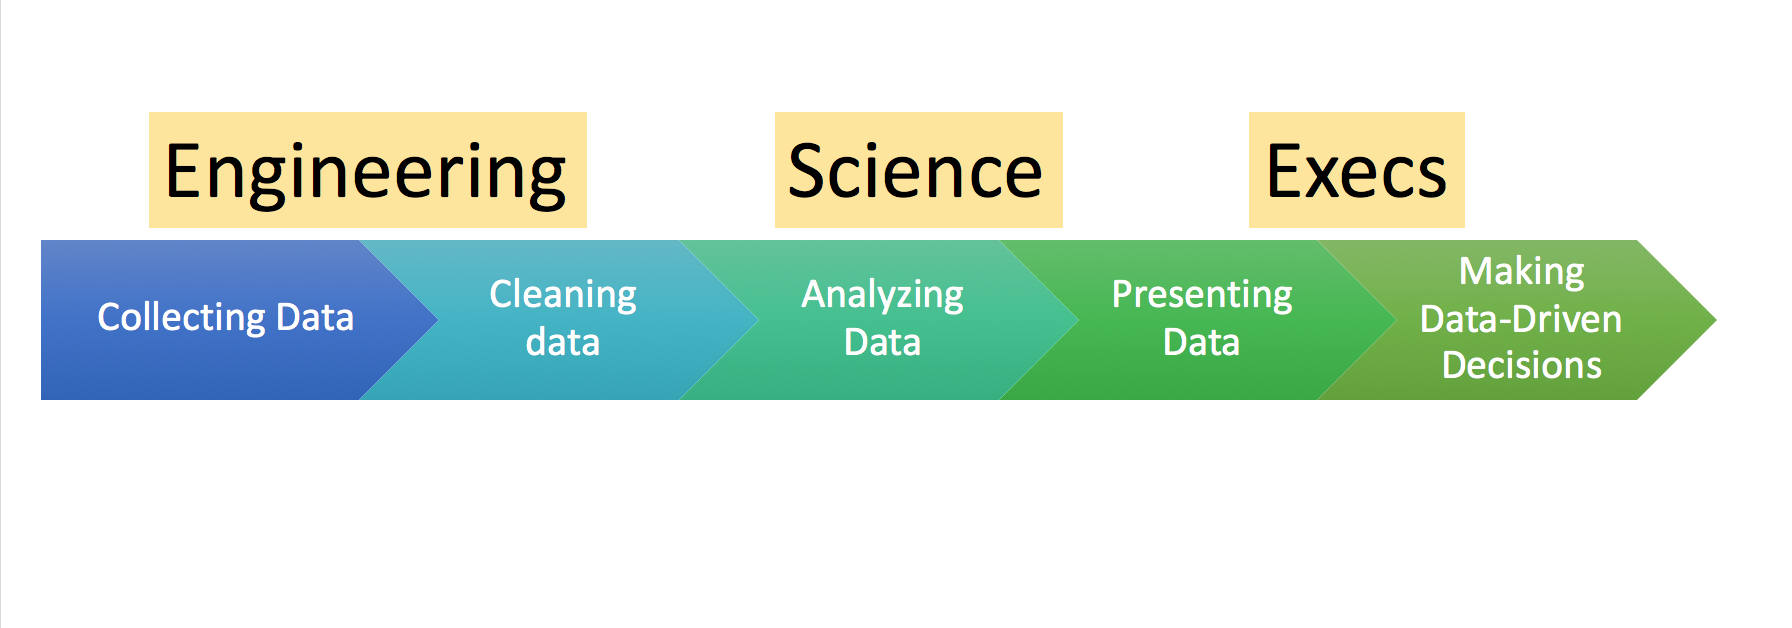
\includegraphics[width=1.1\linewidth]{pipeline}
		%\caption{}
		%\label{fig:datascience}
	\end{figure}
\end{frame}
%%%%%%%%%%%%%%%%%%%%%%%%%%%%%%%%%%%%%%%%%%%%%%%%%
\begin{frame}
	\frametitle{Data science in predictive maintenance: Data engineering}
	\begin{figure}[H]
		\centering
		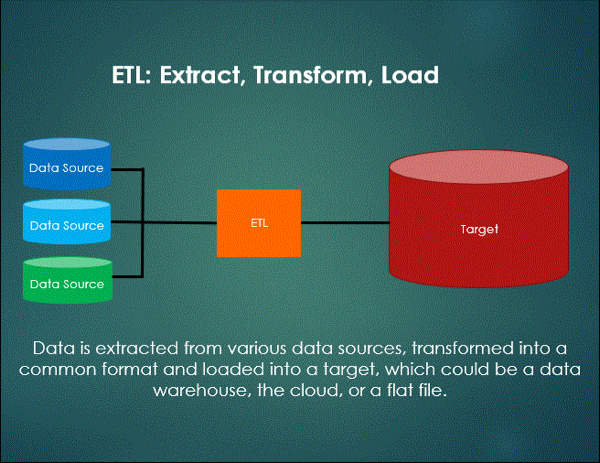
\includegraphics[width=0.55\linewidth]{etl2}
		%\caption{}
		%\label{fig:datascience2}
	\end{figure}
\end{frame}

%%%%%%%%%%%%%%%%%%%%%%%%%%%%%%%%%%%%%%%%%%%%%%%%%
\begin{frame}
	\frametitle{Data science in predictive maintenance: Data cleaning}
	\begin{figure}[H]
		\centering
		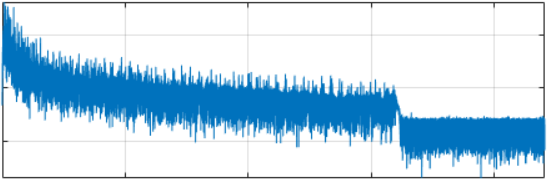
\includegraphics[width=1\linewidth]{vibration}
		%\caption{}
		%\label{fig:datascience}
	\end{figure}
\end{frame}
%%%%%%%%%%%%%%%%%%%%%%%%%%%%%%%%%%%%%%%%%%%%%%%%%%%


\begin{frame}
	\frametitle{Data science in predictive maintenance: Analytics at scale}
	\begin{figure}[H]
		\centering
		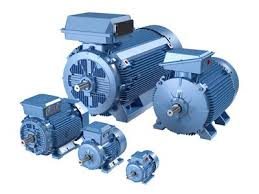
\includegraphics[width=0.2\linewidth]{motor1}
		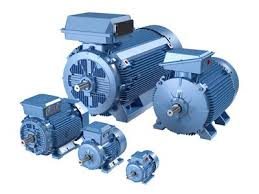
\includegraphics[width=0.2\linewidth]{motor1}
		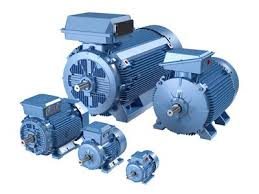
\includegraphics[width=0.2\linewidth]{motor1}
		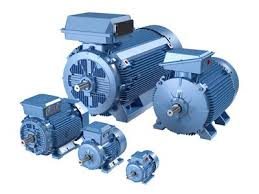
\includegraphics[width=0.2\linewidth]{motor1}
		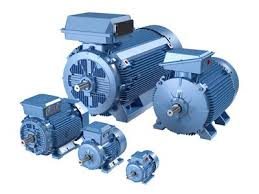
\includegraphics[width=0.2\linewidth]{motor1}
		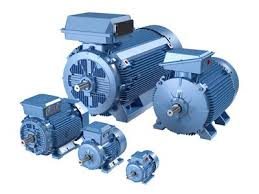
\includegraphics[width=0.2\linewidth]{motor1}
		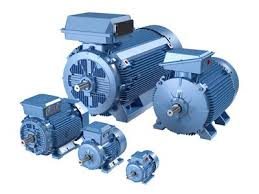
\includegraphics[width=0.2\linewidth]{motor1}
		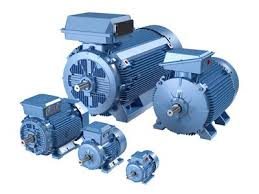
\includegraphics[width=0.2\linewidth]{motor1}
		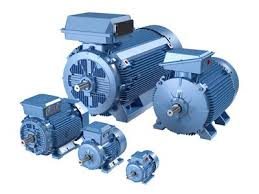
\includegraphics[width=0.2\linewidth]{motor1}
		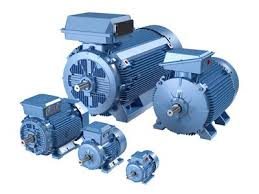
\includegraphics[width=0.2\linewidth]{motor1}
		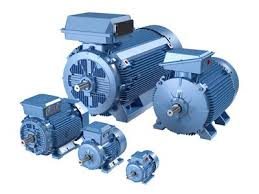
\includegraphics[width=0.2\linewidth]{motor1}
		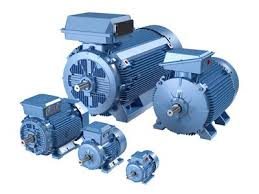
\includegraphics[width=0.2\linewidth]{motor1}
		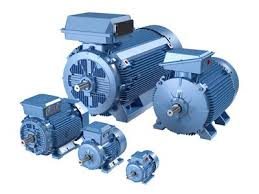
\includegraphics[width=0.2\linewidth]{motor1}
		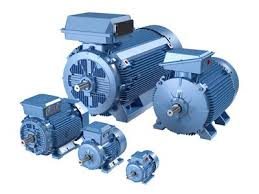
\includegraphics[width=0.2\linewidth]{motor1}
%		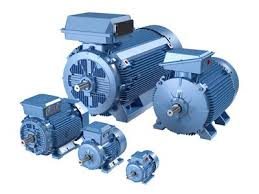
\includegraphics[width=0.2\linewidth]{motor1}
%		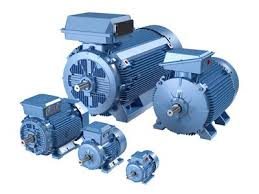
\includegraphics[width=0.2\linewidth]{motor1}
%		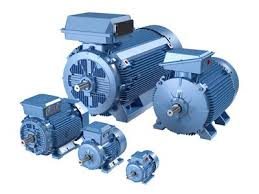
\includegraphics[width=0.2\linewidth]{motor1}
%		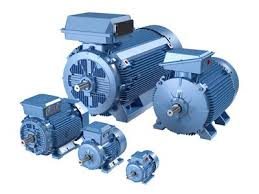
\includegraphics[width=0.2\linewidth]{motor1}
		%\caption{}
	%	\label{fig:datascience}
	\end{figure}
\end{frame}
%%%%%%%%%%%%%%%%%%%%%%%%%%%%%%%%%%%%%%%%%%%%%%%%%%%%%%%%%%%%%%%%%%%%%%%%%%%%%%%%%%%%

\begin{frame}
	\frametitle{Data science in predictive maintenance: Complex machines}
	\begin{figure}[H]
		\centering
		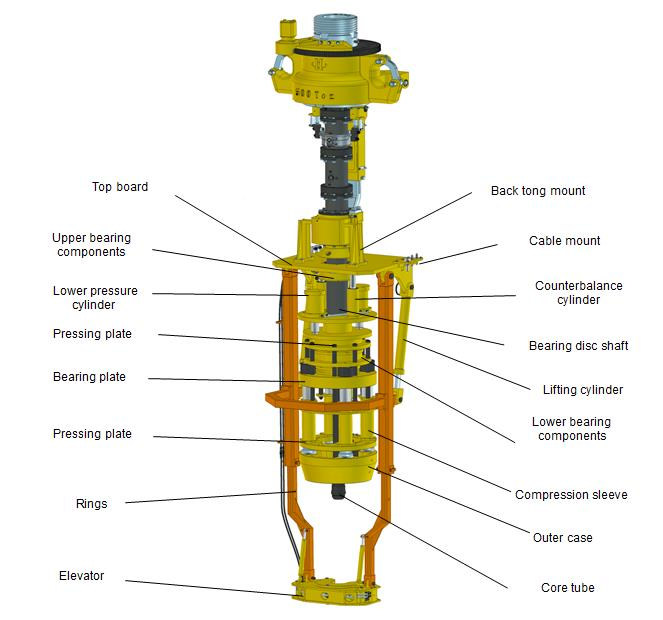
\includegraphics[width=0.5\linewidth]{topdrive}
		%\caption{}
		%\label{fig:datascience}
	\end{figure}
\end{frame}
%%%%%%%%%%%%%%%%%%%%%%%%%%%%%%%%%%%%%%%%%%%%%%%%%%%%%%%%%%%%%%%%%%%%%%%%%%%%%%%
\begin{frame}
	\frametitle{Data science in predictive maintenance: FFT method}
	\begin{figure}[H]
		\centering
		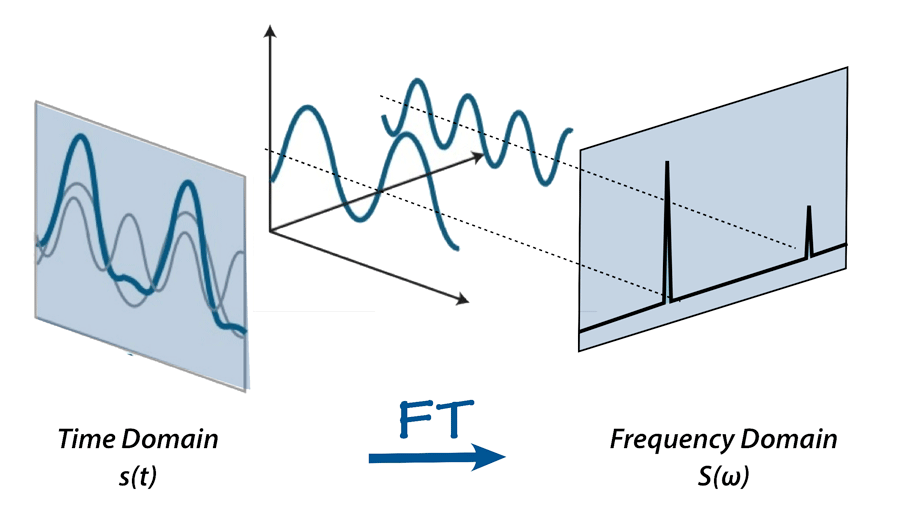
\includegraphics[width=0.4\linewidth]{ft}
		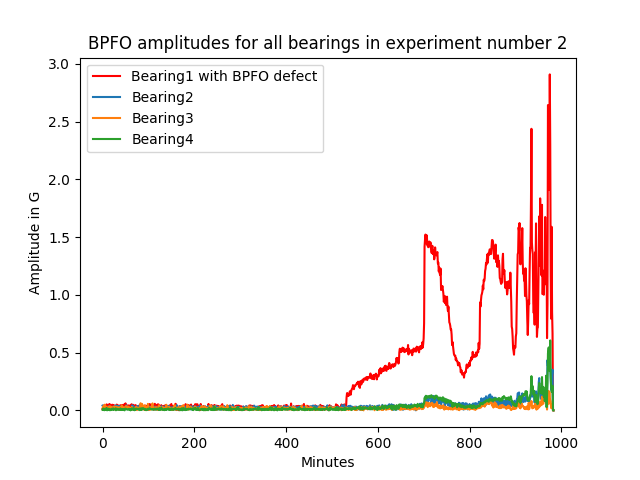
\includegraphics[width=0.4\linewidth]{bpfo}
		%\caption{}
		%\label{fig:datascience}
	\end{figure}
\end{frame}
%%%%%%%%%%%%%%%%%%%%%%%%%%%%%%%%%%%%%%%%%%%%%%%%%%%%%%%%%%%%%%%%%%%%%%%%%%%%%%
\begin{frame}
	\frametitle{Data science in predictive maintenance: Pattern recognition}
	\begin{figure}[H]
		\centering
		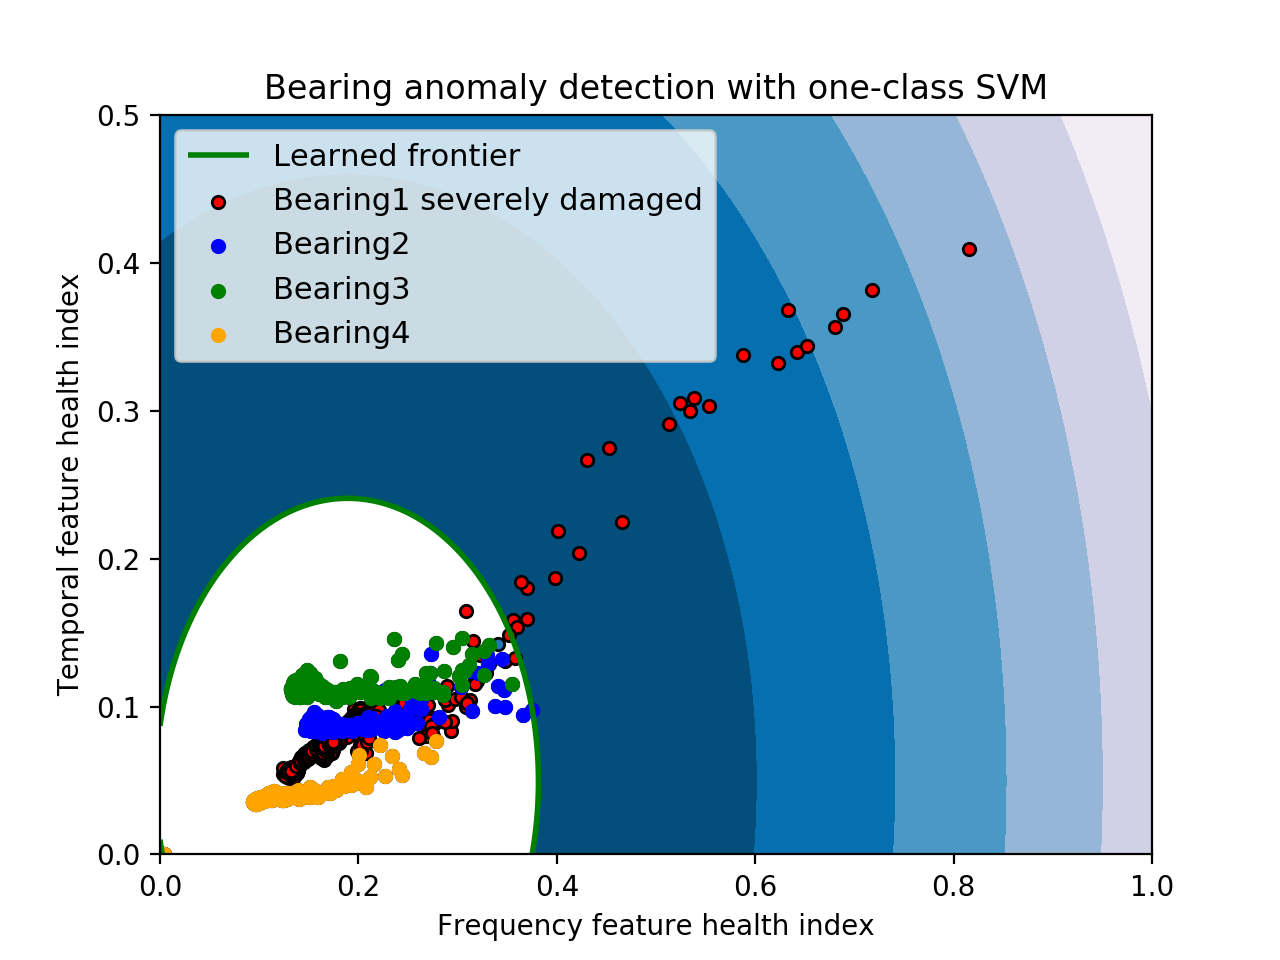
\includegraphics[width=0.6\linewidth]{svm}
		%\caption{}
		%\label{fig:datascience}
	\end{figure}
\end{frame}

%%%%%%%%%%%%%%%%%%%%%%%%%%%%%%%%%%%%%%%%%%%%%%%
\begin{frame}
		\frametitle{Skaiwatch}
		\href{http://skaiwatch.herokuapp.com/dashboardapp/}{Demo}
\end{frame}

\end{document}

